\documentclass[main.tex]{subfiles}

\begin{document}

	\begingroup

	\renewcommand{\cleardoublepage}{}

	\renewcommand{\clearpage}{}

	\chapter{Architecture Overview}
		In order to cope with the challenges we were facing as mentioned in the introduction they have been summarized into five groups:
		\begin{itemize}
			\item Navigation: Movement and localization
			\item Perception: Recognition of objects and classification
			\item Knowledge: Storage and providing access to information about the world state and object positions within the world
			\item Manipulation: Interaction with the world and objects within the world
			\item Planning: Decision making, execution and error handling
		\end{itemize}

		\chapterauthor{}
		
		\section{Diagram}
		
		\begin{figure}	
			\centering
			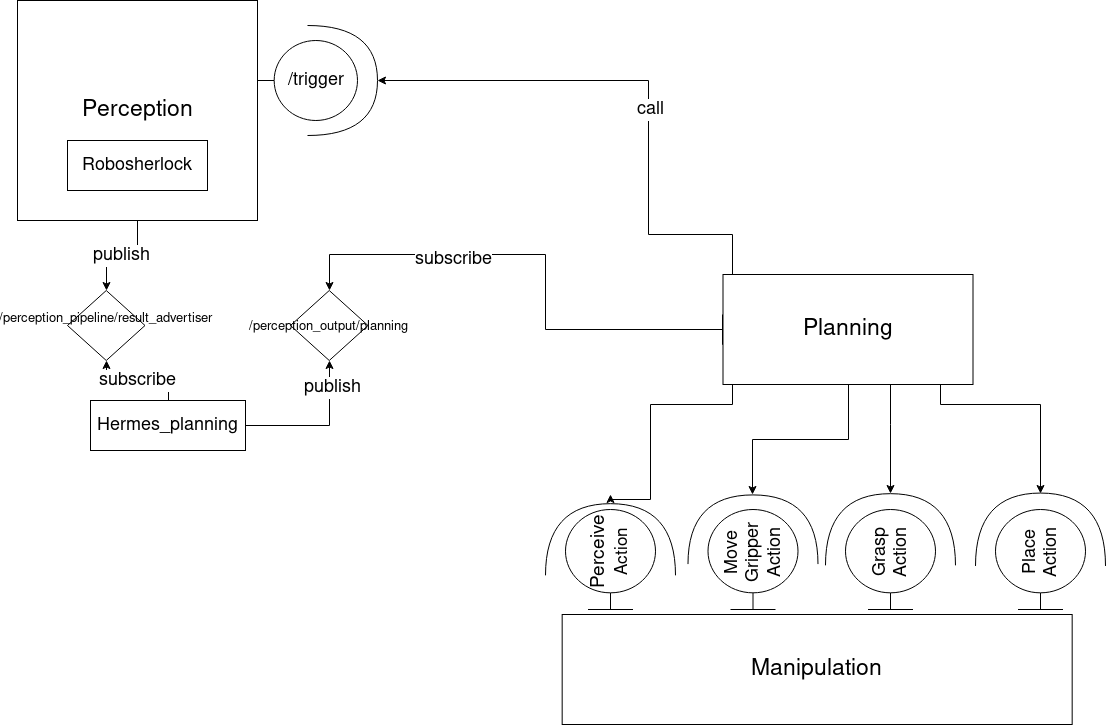
\includegraphics[width=0.85\textwidth]{pictures/diagramms/architecture.png}
			\caption{Architecture overview}
			\label{architecture}
		\end{figure}
		
		\section{Description}
		
			The planning component as seen in \ref{architecture} is basically the connection piece and main executor for the low level robot operations performed by the other components. It basically consists of three packages although the most top level package(execute) was split for the both tasks, the other packages common-functions and low-level-interfacing are explained in following chapters. The planning component initializes connections to the action servers of th other components and sends requests to perform robot actions or as for the access the world representation and knowledge of the robot.
	  		 

	\endgroup

\end{document}
